\chapter{Results and Discussion}
\label{cha:result}
In this section we present a simplified synthetic computer network developed in Python, validating its correctness with respect to our model's assumptions w.r.t queue length stabilization in \cref{sec:Rqueuestabilization}. Once validated we apply baseline techniques introduced in \cref{cha:methodology} to test our new methods for nefarious router identification. We compared these results to previous analytical techniques, highlighting trade offs in accuracy for generally applicability, deploy-ability and run time within \cref{sec:Rnefarouterdetection}. During this analysis several interesting behaviours were encountered in edge cases, these findings are shown and further experiments conducted on hypothesised explanations for the behaviour within \cref{ssec:Rsympathicpdv} and \cref{ssec:Rmetricnormalisation}. Of particular noteworthiness is that the investigation into unexpectedly poor inferential results from router level \pdv  behaviour in \cref{ssec:Rmetricnormalisation} revealed a flaw within previous work's inferential calculation, necessitating changes to the experimental methodology. We then move to testing the impacts of optimal probe allocation techniques on our inferential accuracy in \cref{sec:Rprobingoptimality}, ...\par
\todo{Very brief outline of accuracy changes based on A/D optimality, (it went up/down by x)}
Finally we construct a simulated network using real world topological and traffic data-sets within the NS3 framework to test our new method's performance in real world networks, formulating a quantitative response to our project's overarching goal.

\section{Queue Stabilization}
\label{sec:Rqueuestabilization}

\captionsetup{justification=centering}
\begin{figure}[H]
    \centering
    \begin{subfigure}{0.475\textwidth}
        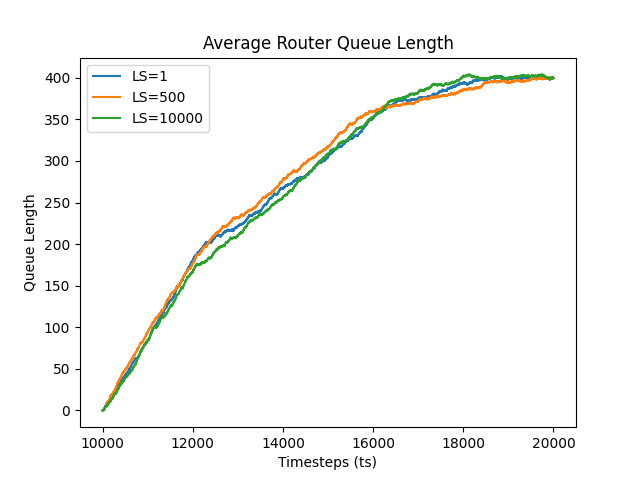
\includegraphics[width=\textwidth]{figs/results/average_of_1,500,10000.png}
        \caption{Average router queue buffer length.}
        \label{fig:Ravgq}
    \end{subfigure}
    \hfill
    \begin{subfigure}{0.475\textwidth}
        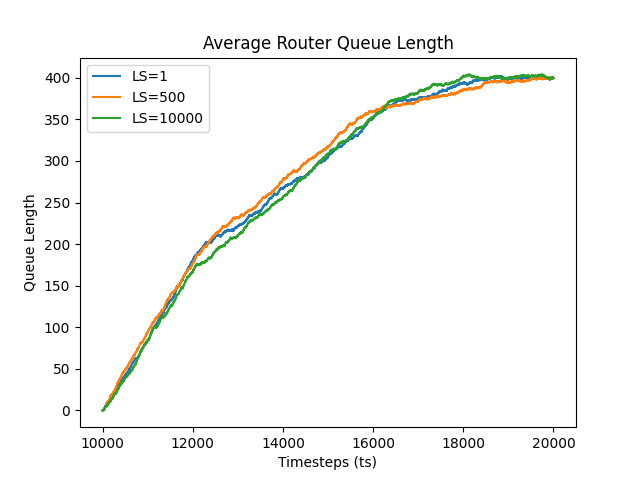
\includegraphics[width=\textwidth]{figs/results/average_of_1,500,10000.png}
        \caption[]{Variance of router queue buffer length.}
        \label{fig:Rvarq}
    \end{subfigure}
    \caption{Mean and variance of router queue buffer lengths over link-state update intervals 1, 500, and 10,000].}
\end{figure}

\begin{table}[H]
    \centering
    \begin{tabular}{||c c c||}
        \hline
        \multicolumn{3}{||c||}{Average Variance Over LS Update Intervals} \\ [0.5ex]
        \hline
        \multicolumn{1}{||c|}{Range} & $ts \leq 20,000$ & $ts > 20,000$ \\ [0.5ex]
        \hline\hline
        1       & 10,657.16 & 6.25 \\ 
        10      & 10,240.66 & 4.88 \\
        50      & 10,128.76 & 3.21 \\
        250     & 10,655.41 & 5.06 \\
        500     & 10,087.16 & 6.05 \\
        1,000   & 10,281.32 & 3.47 \\
        10,000  & 11,169.38 & 5.22 \\ [1ex] 
        \hline
    \end{tabular}
    \caption{Variance pre and post queue length stabilization point}
\end{table}

\section{Nefarious Router Detection}
\label{sec:Rnefarouterdetection}

\subsection*{PDV Inference Validity}
To test our hypothesis that packet delay variation of a router increases proportionally to its probability of nefariously delaying a packet we consider the 6 router network from \cref{sec:Maddtomography} shown in \cref{fig:6routerpdv}. Each trial collected PDV values from   every router each timestep post queue stabilization and then averaged these over a 10,000 timestep simulation run time, these average PDV results from each trial were then averaged over 100 simulations. This process was repeated with nefarious router's holding probability of 0, 0.2, 0.4, 0.6, and 0.8, with four experiments being conducted with router's $r_1$, $r_2$, $r_3$, and $r_4$ being designated nefarious in each experiment respectively, plots of observed PDV can be seen in \cref{fig:MrouterPDV}. From these it is clear that not only does a nefarious router delaying packets increase its 
\begin{figure}
    \centering
    \tikzsetnextfilename{6routerpdvtopology}
    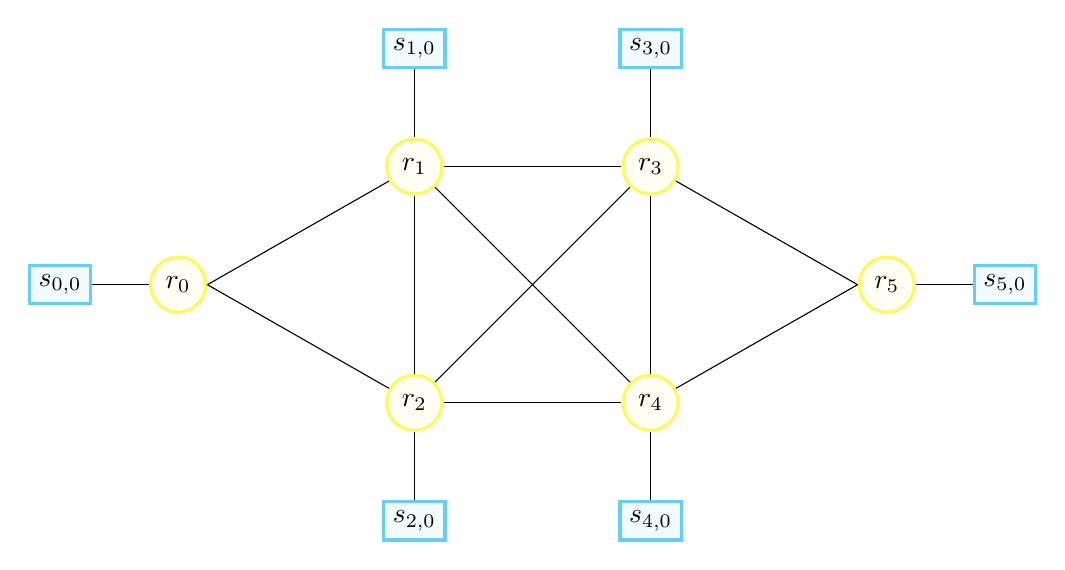
\begin{tikzpicture}[
        router/.style={circle, draw=yellow!60, fill=yellow!5, very thick, minimum size=3.5mm},
        nef_router/.style={circle, draw=red!60, fill=red!5, very thick, minimum size=3.5mm},
        switch/.style={rectangle, draw=cyan!60, fill=cyan!5, very thick, minimum size=2.5mm},
        monitor/.style={rectangle, draw=magenta!60, fill=magenta!5, very thick, minimum size=2.5mm},]
        
        % Routers
        \node[router] (r0) at (-4.5,0)    {$r_0$};
        \node[router] (r1) at (-1.5,1.5)  {$r_1$};
        \node[router] (r2) at (-1.5,-1.5) {$r_2$};
        \node[router] (r3) at (1.5,1.5)   {$r_3$};
        \node[router] (r4) at (1.5,-1.5)  {$r_4$};
        \node[router] (r5) at (4.5,0)     {$r_5$};
        
        %Switches
        \node[switch](s00) at (-6,0)   {$s_{0,0}$};
        \node[switch] (s10) at (-1.5,3)   {$s_{1,0}$};
        \node[switch] (s20) at (-1.5,-3)  {$s_{2,0}$};
        \node[switch] (s30) at (1.5,3)   {$s_{3,0}$};
        \node[switch] (s40) at (1.5,-3)   {$s_{4,0}$};
        \node[switch] (s50) at (6,0)   {$s_{5,0}$};
        %Links
        \draw[-] (r0.east) -- (r1);
        \draw[-] (r0.east) -- (r2);
        \draw[-] (r1) -- (r2);
        \draw[-] (r1) -- (r3);
        \draw[-] (r1.south east) -- (r4.north west);
        \draw[-] (r2) -- (r3);
        \draw[-] (r2) -- (r4);
        \draw[-] (r3) -- (r4);
        \draw[-] (r3) -- (r5.west);
        \draw[-] (r4) -- (r5.west);
        \draw[-] (s00.east) -- (r0.west);
        \draw[-] (s10) -- (r1);
        \draw[-] (s20) -- (r2);
        \draw[-] (s30) -- (r3);
        \draw[-] (s40) -- (r4);
        \draw[-] (s50.west) -- (r5.east);
    \end{tikzpicture}
    \caption{6 router network.}
    \label{fig:6routerpdv}
\end{figure}

\begin{figure}
    \centering
    \begin{subfigure}{0.475\textwidth}
        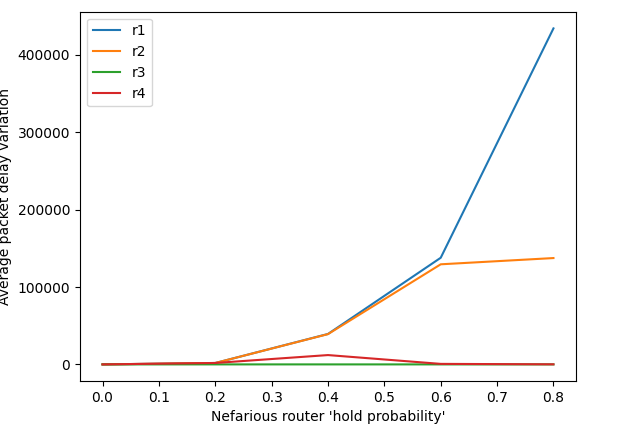
\includegraphics[width=\textwidth]{figs/results/true_PDV_1.png}
        \caption[]{$r_1$ nefarious.}
    \end{subfigure}
    \begin{subfigure}{0.475\textwidth}
        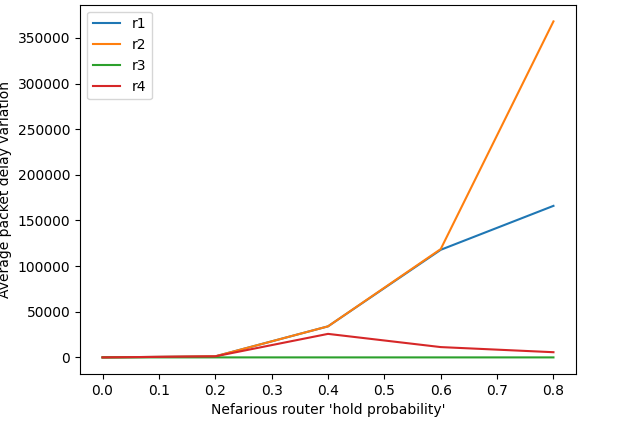
\includegraphics[width=\textwidth]{figs/results/true_PDV_2.png}
        \caption[]{$r_2$ is nefarious.}
    \end{subfigure}
    \hfill
    \centering
    \begin{subfigure}{0.475\textwidth}
        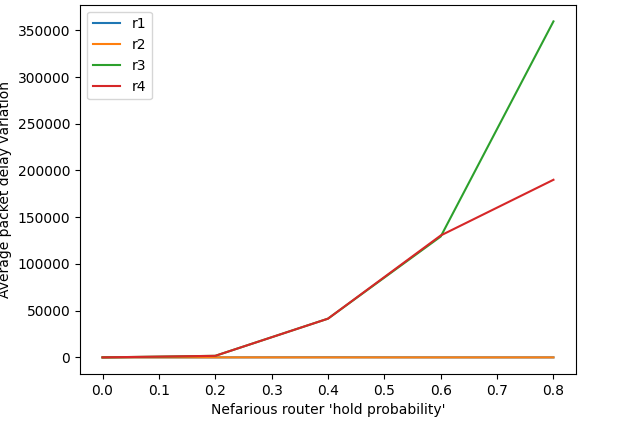
\includegraphics[width=\textwidth]{figs/results/true_PDV_3.png}
        \caption[]{$r_3$ nefarious.}
    \end{subfigure}
    \begin{subfigure}{0.475\textwidth}
        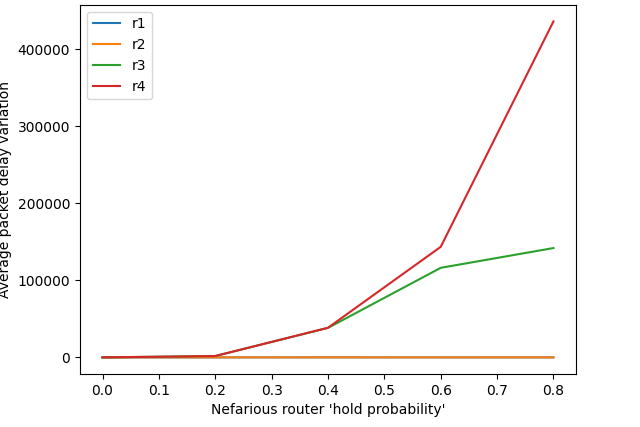
\includegraphics[width=\textwidth]{figs/results/true_PDV_4.png}
        \caption[]{$r_4$ nefarious.}
    \end{subfigure}
    \caption[Results of router level PDV over varying hold probabilities.]{Average PDV over varying nefarious holding probabilities.}
    \label{fig:MrouterPDV}
\end{figure}

\subsection*{Sympathetic PDV Increase}
\label{ssec:Rsympathicpdv}

\subsection*{Tomographic Inference Accuracy}
\begin{figure}[H]
        \centering
        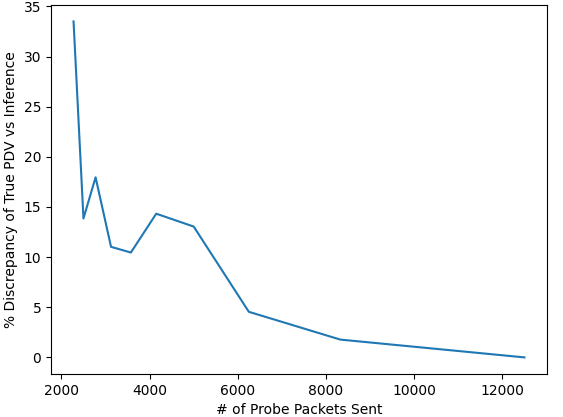
\includegraphics[width=\textwidth]{figs/results/Probe_PDV_accuracy_plot.png}
        \caption{Accuracy of inference from true values over a range of probes sent.}
        \label{fig:Rqstabilization}
\end{figure}
\emph{Cover results in a 7 router network and resulting metric normalisation (refer to \cref{ssec:Rsympathicpdv} for 6 router) and 10 router, then for novel topologies (Peterson graph, tripartite graph)}


\subsection{Metric Normalisation}
\label{ssec:Rmetricnormalisation}
The delay distribution and by extension delay variation at a single router is intuitively a combination of the two contributors to \gls{qlen} within the system:
\begin{enumerate}
    \item The \# of packets a router receives.
    \item The \# of packets a router sends.
\end{enumerate}
Contributor \emph{2} is always a fixed rate of 1 packet per time step unless a router is nefarious in which case it will be $<1$ proportional to the router's probability of holding a packet. As the rate of sending is not impacted by contributor \emph{1} we account for variation of contributor \emph{1} between routers to increase the transparency of queuing delay due to variations by contributor \emph{2} within the network.\par
The variation in contributor \emph{1} is proportional to the degree of each node as the number of packets being received by a router each time step is the sum of packets received from each link. Initially we utilized $\sqrt{\gls{routerdeg}}$ for normalization over delay observations by taking $\forall r\in R, \frac{\sigma^2}{\sqrt{\gls{routerdeg}}}$ where $\sigma^2$ is the variance of delay measurements.
\todo{Show results for inferential accuracy RE probing a network where nefarious router has << switches than a non-nef, to demonstrates why we want to normalise for the number of links. }

\section{Probing Optimality}
\label{sec:Rprobingoptimality}

\section{Real Network Performance}
\label{sec:Rrealnetworkperformance}

\section{Summary}
